%% Copernicus Publications Manuscript Preparation Template for LaTeX Submissions
%% ---------------------------------
%% This template should be used for copernicus.cls
%% The class file and some style files are bundled in the Copernicus Latex Package, which can be downloaded from the different journal webpages.
%% For further assistance please contact Copernicus Publications at: production@copernicus.org
%% https://publications.copernicus.org/for_authors/manuscript_preparation.html


%% Please use the following documentclass and journal abbreviations for preprints and final revised papers.

%% 2-column papers and preprints
\documentclass[amt, article]{copernicus}
\usepackage[utf8]{inputenc}
\usepackage{subcaption}
\usepackage{natbib}
\bibliographystyle{copernicus}
\usepackage{hyperref}    % Create hyperlinks
\usepackage{xcolor}
\hypersetup{
    colorlinks,
    linkcolor={red!50!black},
    citecolor={red!50!black},
    urlcolor={red!80!black}
}
%\usepackage[switch]{lineno}
%\usepackage{siunitx,etoolbox}
%% Journal abbreviations (please use the same for preprints and final revised papers)


% Advances in Geosciences (adgeo)
% Advances in Radio Science (ars)
% Advances in Science and Research (asr)
% Advances in Statistical Climatology, Meteorology and Oceanography (ascmo)
% Aerosol Research (ar)
% Annales Geophysicae (angeo)
% Archives Animal Breeding (aab)
% Atmospheric Chemistry and Physics (acp)
% Atmospheric Measurement Techniques (amt)
% Biogeosciences (bg)
% Climate of the Past (cp)
% DEUQUA Special Publications (deuquasp)
% Earth Surface Dynamics (esurf)
% Earth System Dynamics (esd)
% Earth System Science Data (essd)
% E&G Quaternary Science Journal (egqsj)
% EGUsphere (egusphere) | This is only for EGUsphere preprints submitted without relation to an EGU journal.
% European Journal of Mineralogy (ejm)
% Fossil Record (fr)
% Geochronology (gchron)
% Geographica Helvetica (gh)
% Geoscience Communication (gc)
% Geoscientific Instrumentation, Methods and Data Systems (gi)
% Geoscientific Model Development (gmd)
% History of Geo- and Space Sciences (hgss)
% Hydrology and Earth System Sciences (hess)
% Journal of Bone and Joint Infection (jbji)
% Journal of Micropalaeontology (jm)
% Journal of Sensors and Sensor Systems (jsss)
% Magnetic Resonance (mr)
% Mechanical Sciences (ms)
% Natural Hazards and Earth System Sciences (nhess)
% Nonlinear Processes in Geophysics (npg)
% Ocean Science (os)
% Polarforschung - Journal of the German Society for Polar Research (polf)
% Primate Biology (pb)
% Proceedings of the International Association of Hydrological Sciences (piahs)
% Safety of Nuclear Waste Disposal (sand)
% Scientific Drilling (sd)
% SOIL (soil)
% Solid Earth (se)
% State of the Planet (sp)
% The Cryosphere (tc)
% Weather and Climate Dynamics (wcd)
% Web Ecology (we)
% Wind Energy Science (wes)


%% \usepackage commands included in the copernicus.cls:
%\usepackage[german, english]{babel}
%\usepackage{tabularx}
%\usepackage{cancel}
%\usepackage{multirow}
%\usepackage{supertabular}
%\usepackage{algorithmic}
%\usepackage{algorithm}
%\usepackage{amsthm}
%\usepackage{float}
%\usepackage{subfig}
%\usepackage{rotating}


\begin{document}

\title{IRIS-CloudDeep: Infrared Radiometric Image classification and Segmentation of Cloud structure using Deep-learning framework for ground-based long-wave infrared thermal camera observation}


% \Author[affil]{given_name}{surname}

\Author[1,*]{Kélian}{Sommer}
\Author[2,*]{Wassim}{Kabalan}
\Author[3,*]{Romain}{Brunet}

\affil[1]{Laboratoire Univers et Particules de Montpellier, Université de Montpellier, CNRS, Montpellier, France}
\affil[2]{APC, Univ Paris Diderot, CNRS/IN2P3, CEA/lrfu, Obs de Paris, Sorbonne Paris Cité, France}
\affil[3]{Laboratoire d’Astrophysique de Marseille, Marseille, France}

%% The [] brackets identify the author with the corresponding affiliation. 1, 2, 3, etc. should be inserted.

%% If an author is deceased, please mark the respective author name(s) with a dagger, e.g. "\Author[2,$\dag$]{Anton}{Smith}", and add a further "\affil[$\dag$]{deceased, 1 July 2019}".

%% If authors contributed equally, please mark the respective author names with an asterisk, e.g. "\Author[2,*]{Anton}{Smith}" and "\Author[3,*]{Bradley}{Miller}" and add a further affiliation: "\affil[*]{These authors contributed equally to this work.}".


\correspondence{Kélian Sommer (kelian.sommer@umontpellier.fr), Wassim Kabalan (wassim.kabalan@apc.in2p3.fr) and Romain Brunet (romain.brunet@lam.fr)}

\runningtitle{Infrared Radiometric Image classification and Segmentation of Cloud structure}

\runningauthor{K. Sommer et al.}

\received{}
\pubdiscuss{} %% only important for two-stage journals
\revised{}
\accepted{}
\published{}

%% These dates will be inserted by Copernicus Publications during the typesetting process.


\firstpage{1}

\maketitle



\begin{abstract}
    Infrared thermal cameras offer reliable means of assessing atmospheric conditions by measuring the downard radiance from the sky, facilitating their usage in cloud monitoring endeavors. Precise identification and detection of clouds in images poses great challenges stemming from the indistinct boundaries inherent to cloud formations. Various methodologies for segmentation have been previously suggested. Most of them rely on color as the distinguishing criterion for cloud identification in the visible spectral domain and thus lack the ability to detect cloud structure on gray-scaled images with satfisactory accuracy. In this work, we propose a new complete deep-learning architecture to perform image classification based on a Convolutional Neural Network (CNN) and image segmentation by exploring the use of U-Net encode/decoder model. We demonstrate the effectiveness of this technique by conducting a series of tests and validation on self-captured infrared sky images and transformed publicly available datasets. We find that the models accurately discriminate image types and capture precise cloud structure information even when trained with single ground truth per input sample. We also show that our method achieves better overall performance than other state-of-the-art methods. We emphasize that our framework offers strong viability and can be used for sustained cloud monitoring operations over extended durations.
\end{abstract}

%\copyrightstatement{TEXT} %% This section is optional and can be used for copyright transfers.


\introduction  %% \introduction[modified heading if necessary]

% INTEREST OF CLOUDS IN GENERAL
Accurate and continuous monitoring of cloud properties contributes to a profound understanding of atmospheric processes and their subsequent impacts on various Earth systems \citep{liou1992radiation}. It provides essential insights for weather predictions and climate dynamics \citep{hu2004application,petzold2015global}.

% WAYS OF CLOUD OBSERVATION
Many diverse instruments are dedicated towards cloud detection and associated observation methods can be divided into two primary distinct categories: downward satellite-based observations \citep{roy2017satellite, martin2008satellite} and upward ground-based observations \citep{wilczak1996ground} (e.g. all-sky cameras, lidar, radar). The principal aim of satellite-based observations is to investigate the upper regions of clouds, facilitating the examination and analysis of global atmospheric patterns and climate conditions over expansive geographical areas \citep{schiffer1983international, boers2006satellite, geer2017growing, varnai2018satellite}. In contrast, ground-based cloud observation excels in the surveillance of localized regions, furnishing valuable data pertaining to the lower segments of clouds (e.g. information on cloud altitude, cloud extent, and cloud typology) \citep{bower2000ace, zhou2019cloud}. Complementarity of these two types of measurement techniques allow better understanding of cloud behaviour in general \citep{mokhov1994analysis, schreiner1993comparison, yamashita2012ground, yoshimura2013contribution}.

% MORE ABOUT GROUND BASED OBSERVATIONS
Ground-based observations have been extensively used in recent years and has become one of the primary means to studying cloud formations \citep{paczynski2000monitoring}. As technological evolution has ushered in a new era of observation methodologies \citep{mandat2014all}, the utilization of infrared thermal cameras has emerged as a promising avenue for atmospheric investigations through precise radiometric measurements \citep{Szejwach1982, Shaw_2013, liandrat2017cloud, lopez2017contribution, Klebe2014, nikolenko2021infrared}.
%applications in many domains such as medicine \citep{ring2012infrared}, agriculture \citep{ishimwe2014applications}, military defence \citep{akula2011thermal} and surveillance systems \citep{wong2009effective}.
Because of their practical use, high sensitivity, low-cost, operating range and wide field-of-view (FOV) \citep{Rogalski2011,Rogalski2014,Kimata2018}, it makes them particularly useful for aerial \citep{wilczak1996ground}, defense \citep{gallo1993low}, weather forecast \citep{sun2008whole, Liandrat2017} or even astronomical applications \citep{Klebe2010,Klebe2012,Klebe2014} to determine the cloud cover fraction during operations and therefore assess the quality of scientific observations. Indeed, uncooled infrared microbolometers array sensors working in the 10-12 $\mu m$ spectral band can directly detect the LWIR emission of both clouds and the atmospheric background, excluding the scattered light of the sun or starlight \citep{Houghton1972}.
%Contrary to cameras operating in the visible spectrum, these LWIR sensors are able to provide reliable measurements of cloud properties at night. 
Across recent years, multiple automatic ground-based observations systems have been developed. For example, the infrared cloud imager (ICI) \citep{ICI}, can detect clouds and assess cloud coverage both in daylight and at nighttime with a dedicated infrared sensor. \citet{Sharma2015} designed an instrument to detect of the cloud infrared radiations to be used in search for a potential site for India’s National Large Optical Telescope project.
%The ICI functions as a passive instrument, measuring the downward atmospheric radiance through a relatively narrow field of view (FOV) measuring about 250 deg$^{2}$ at a resolution of 320 $\times$ 240 pixels.
The all-sky infrared visible analyzer (ASIVA) \citep{Klebe2014} represents a distinctive device capable of acquiring an extensive field of view (FOV) infrared sky image without the need for a scanning mechanism. The ASC-200 system \citep{rs13091852} combines information from two all-sky cameras facing the sky operating in both the visible spectrum (450-650 nm) and the LWIR band (8-14 $\mu m$), called the TIRASVC instrument). It features a thermal microbolometer array sensitive to radiation in the 8–14 $\mu m$ spectral range and a specifically designed wide-angle germanium lens.

% RELATION TO ASTRONOMY
As next-generation cosmological surveys require more demanding precision on photometric observations (implying better characterization of the atmosphere), monitoring instruments field-of-view (FOV) with LWIR thermal cameras may provide significant asset to estimate cloud coverage, precipitable water vapor content (PWV) and classify observations quality. Multiple ground-based all-sky and narrow field-of-view (FOV) infrared instruments have demonstrated reliable measurements of sky radiance \citep{Klebe2012, Klebe2014}.
%For the upcoming Vera Rubin Observatory cosmological survey, preliminary work has demonstrated the feasability to monitor the entire sky with uncooled infrared cameras. 

In this study, we use a similar infrared sensor with a narrower FOV (i.e. 60 mm F1.25 germanium athermal lens) that aims to monitor a high-sensivity photometric telescope line of sight for astronomical purposes. It is part of the StarDICE metrology experiment \citep{stardice1} that aims at measuring CALSPEC \citep{Bohlin2014} spectrophotometric reference stars flux at the 0.1\% relative uncertainty level. Enhanced characterization of atmospheric conditions are required to reach the target sensitivity. As a first step, basic indication of the atmosphere conditions in the telescope FOV may provide valuable insights onto the quality of spectrophotometric measurements. However, these kind of instruments operate at high framerate and produce considerable amounts of data which make it extremely difficult to analyze by human observers. Therefore, to determine cloud presence in infrared images, deep convolutional neural networks appear to be a viable approach to process images in real-time. Inspired by large successes encountered in image classification and structure detection for various computer vision tasks, multiple models relying on convolutional neural network (CNN) have been developed, including: CloudSegnet \citep{dev2019cloudsegnet}, CloudU-Net \citep{CloudUNet} CloudU-Netv2 \citep{CloudUNetv2}, SegCloud \citep{SegCloud}, TransCloudSeg \citep{TransCloudSeg}, CloudDeepLabV3 \citep{CloudDeepLabV3}, ACLNet \citep{makwana2022aclnet}, DeepCloud \citep{DeepCloud}, CloudRaednet \citep{shi2022cloudraednet}, DMNet \citep{DMNet} and DPNet \cite{DPNet}.
Others are specifically dedicated toward satellite imagery \cite{kim2018deep, kanu2020cloudx, chen2023novel}. Majority of these models are typically structured using an encoder–decoder architecture, with the encoder incorporating CNNs \citep{oshea2015introduction}. The encoder's role is to capture both high-level and low-resolution features, while the decoder generates the segmentation mask \citep{badrinarayanan2017segnet, Alzubaidi2021ReviewOD}. Nonetheless, these methodologies exclusively address RGB-colored images. Colors (or HUE) provides the essential of information for segmentation (especially red and blue channels). In the case of LWIR thermal images, we need to use a dedicated model capable of achieving comparable accuracy for single-channel gray-scaled images. Consequently, we develop a deep-learning framework designed to: (i) classify images (e.g, detect if any cloud is present onto the image and discriminates between clear and cloudy images); (ii) identify cloud structure (e.g., generate a pixel-based probabilistic segmentation map and verify if the CCD camera FOV is impacted).
The main contributions of this paper are threefold:
\begin{itemize}
    \item IRIS-CloudDeep: new infrared sky image classification and cloud segmentation using deep-learning framework for ground-based radiometric camera observation;
    \item Comparison of the proposed solution to various state-of-the-art methods;
    \item Viable method for vetting astronomical observations quality in real-time.
\end{itemize}
The source code and supporting materials of IRIS-CloudDeep are available online at \url{https://github.com/kelian98/IRIS-CloudDeep}.
The remainder of the paper is organized as follows. Some background about the scientific context of the StarDICE metrology experiment and related works is presented in Section 3. Section 3 details the experimental setup and dataset. Section 4 introduces the proposed framework, describing deep-learning architectures and training procedures. Experimental results and comparisons with other methods are provided in Section 5. Relevant matters and future perspectives are discussed in Section 6. Section 7 depicts a summary and finally concludes the paper.

\section{Background}

\subsection{Motivation}

StarDICE represents one of the initiatives focused on creating a measurement process that bridges the gap between laboratory flux standards (such as silicon photodiodes calibrated by NIST) and the stars found in the CALSPEC library of spectrophotometric references \citep{Bohlin2020}. Since supernova surveys rely on the calibration of these standard stars for their measurements, successfully establishing this connection with high precision effectively addresses the calibration challenge associated with the Hubble diagram. The StarDICE proposal encompasses a five-step sequence, as illustrated in Figure \ref{fig:schematics_stardice}. This process hinges on the near-field calibration of an exceptionally dim light source, emitting less than 1 $\mu$W of optical power, and known for its stability. This calibrated light source, in turn, serves as a distant ($\sim$ 100 m) in-situ reference for a compact astronomical telescope.
One of the largest remaining source of systematic uncertainty is Earth atmosphere transmission \citep{stubbs2012addressing, Stubbs2015, Li2016}. It is dependent on many environmental conditions and processes, including: absorption and scattering (Rayleigh) by molecular constituents (O2, O3, and other elements), absorption by precipitable water vapor (PWV), scattering (Mie) by optical wavelength sized aerosols particles, and shadowing by larger ice crystals and water droplets in clouds that is independent of wavelength (gray) \citep{Burke2010, Burke2017}. Current atmospheric transmission or extinction models do not integrate the possible impact of cloud. Indeed, formation of thin clouds through the condensation of water droplets and ice can result in clouds that are extremely faint and cannot be perceived in the visible spectrum with the naked eye. These clouds often exhibit complex spatial structures, as demonstrated in \citet{Burke2014}. The condensation process takes place along well-defined boundaries in temperature and pressure, which are influenced by the volume density of Precipitable Water Vapor (PWV). This phenomenon commonly categorizes observing conditions as either \textit{photometric} or \textit{non-photometric}.
To address this issue, we propose to use an infrared thermal camera providing high-sensitivity radiometric measurements of the sky radiance in the atmosphere transparency window. Previous work demonstrated our ability to calibrate it with better than 0.1 $W/m^{2}/sr$ on each pixel, corresponding to the added radiance of a theoretical cirrus cloud at surface temperature of 205 K with a visible optical depth of $\tau$ = 0.02. This device may be the key to assess photometric observations quality and label science images with superior than state-of-the-art accuracy.

\begin{figure}[t]
	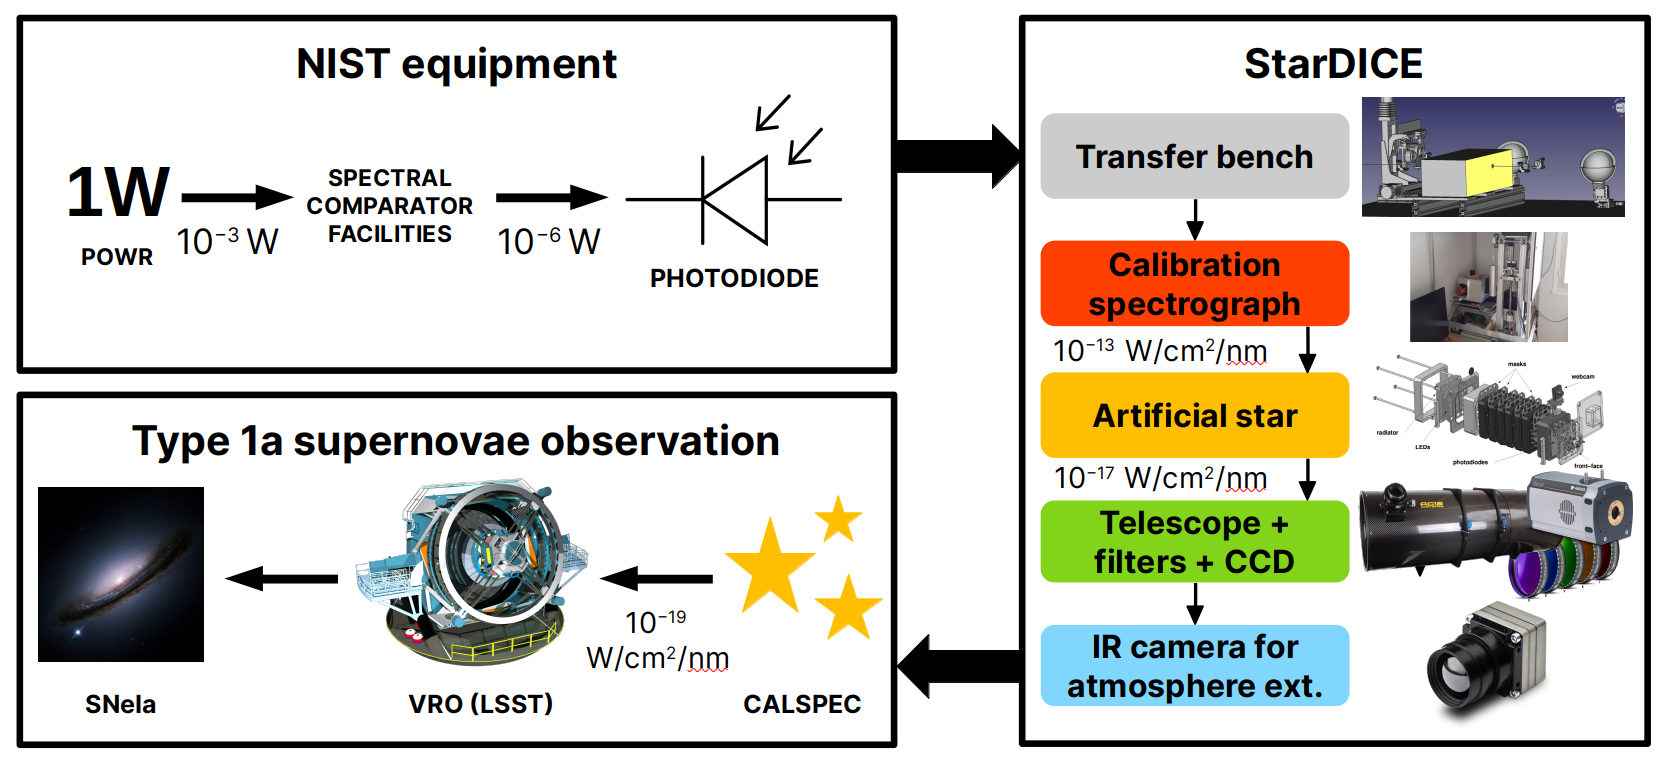
\includegraphics[width=\hsize]{figures/schematics_stardice.png}
	\caption{Schematics of the metrology chain of the StarDICE experiment. Each arrow represents a step in the chain and the label gives the order of magnitude of the beam intensity. The steps in upper left box are conducted at NIST \citep{Larason2008} and result in a silicon photodiode calibrated against an electrical substitution cryogenic radiometer. The StarDICE collaboration builds the dedicated bench transfer system in the right box, designed to reach $10^{-19} \: W/cm2/nm$ flux sensitivity. Primary calibration stars catalog is then used by large cosmological surveys for absolute flux calibration.}
    \label{fig:schematics_stardice}
\end{figure}

\subsection{Related work}

In recent years, numerous cloud sky/cloud segmentation algorithms have been introduced along with the increased development of all-sky ground-based cloud monitoring stations \citep{Long2006, Yang2012, rs12111902, ASC2, amt-15-3629-2022}.
Indeed, cloud segmentation is big challenge for remote sensing applications as cloud comes in various shapes and forms. Therefore, the most modern common approach aims to use computer vision encoder-decoder architectures algorithms and train them onto very specific publicly available cloud images database such as: SWIMSEG, SWINSEG, SWINySEG (combination of both), WSISEG, HYTA and TLCDD. Most proposed solutions are focus on visible RGB images.
CloudSegNet \citep{dev2019cloudsegnet} is a light-weight deep-learning encoder/decoder network that detects clouds onto daytime and nighttime visible color images.
CloudU-Net \citep{CloudUNet} modifies CloudSegNet architecture by adding dilated convolution, skip connection, and fully connected conditional random field (CRF, see \citet{McCallumCRF}) layers to demonstrates better segmentation performance overall. It uses the powerful U-Net architecture \citep{UNET} originally applied to medical image segmentation.
CloudU-Netv2 \citep{CloudUNetv2} replaces the upsampling in CloudU-Net with bilinear upsampling, improves discrimination ability of features representation and uses rectified Adam (rADAM is a variant of the Adam \cite{ADAM} stochastic optimizer that introduces a term to rectify the variance of the adaptive learning rate, see \citet{RADAM}) as the optimizer.
SegCloud \citep{SegCloud} has been trained onto 400 images and possesses a symmetric encoder–decoder structure and outputs low/high-level cloud feature maps to the same resolution of input images.
TransCloudSeg \citep{TransCloudSeg} adresses the loss of global information due to limited receptive field size of the filters in CNN by proposing an hybrid model containing both the CNN and a transformer \citep{TRANSFORMER} as the encoders to obtain different features.
CloudDeepLabV3+ \citep{CloudDeepLabV3} designs a lightweight ground-based cloud image adaptive segmentation method  that integrates multi-scale fea­tures aggregation and multi-level attention feature enhancement.
ACLNet \citep{makwana2022aclnet} uses EfficientNet-B0 as the backbone, “à trous spatial pyramid pooling” (ASPP see \citet{ATROUS}) to learn at multiple receptive fields, and “global attention module” (GAM see \citet{GAM}) to extract fine-grained details from the image. It provides lower error rate, higher recall and higher F1-score than state-of-art cloud segmentation models.
DeepCloud \citep{DeepCloud} uses the method of Fisher vector encoding which is applied to executing the spatial feature aggregation and high-dimensional feature mapping on the raw deep convolutional features.
CloudRaednet \citep{shi2022cloudraednet} proposes a residual attention-based encoder–decoder network and train it over the SWINySEG dataset.
\citep{MACNN} introduces a novel deep model named multiscale attention convolutional neural network (MACNN) to obtain different receptive fields by using different hole rates for the filters and propose the attention module to learn the attention coefficients in order to reflect different importance of pixels.
DMNet \citep{DMNet} proposes a novel cloud detection network that aims to achieve information complementarity by exploiting the different properties of the features at different levels of the encoder, so as to strengthen the detailed information of high-level features and make the low-level features have more semantics.
DPNet \citep{DPNet} possesses an encoder-decoder structure
with Dual Pyramid Pooling Module (DPPM). Specifically, they process the feature maps of different scales in the encoder through a technique known as dual pyramid pooling. They also implement the Encoder-Decoder Constraint (EDC) to relieve information loss in the process of encoding and decoding.

Overall, the primary innovation brought forth by CNN-based approaches in the realm of ground-based cloud image segmentation is the introduction of the encoder–decoder architecture. The encoder is tailored to acquire representational features, facilitating the extraction of semantic information. Subsequently, the decoder reconstructs these representational features into the segmentation mask, allowing for pixel-level classification.

Others have proposed solutions for all-sky infrared image classification.
\citet{Liu2021} applies pre-processing steps (smoothing noise reduction, enhancement through top-hat transformation and a high-pass filtering, edges detection) before extracting features that are useful for distinguishing cirriform, cumuliform, and waveform clouds. A simple rectangle method as supervised classifier is applied. They find a 90\% agreement between a priori classificatoin carried out manually by visual inspection and their algorithm on 277 images. \citet{SUN2011278} suggested: (i) a method for determining clear sky radiance threshold; (ii) cloud identification combined threshold method with texture method; (iii) an algorithm to retrieve cloud base height from downwelling infrared radiance. They showed that structural features are better than texture features in classifying cloud. \citet{amt-11-5351-2018} proposed a three-step process: (i) pre-processing; (ii) feature extraction; (iii) classification method to group images into five cloud categories (stratiform, cumuliform, waveform, cirriform and clear) based on manifold and texture features using support vector machine (SVM). Their experimental results demonstrate the higher recognition rate with an increase of 2\%–10\% on ground-based infrared images datasets. Nevertheless, these methods class clouds into separate categories based on their typology. Until now, all the previously examined approaches, while effective within their specific domains, proved to be unsuccessful when applied to our particular use case. Therefore, we propose a new deep-learning framework based on CNNs and U-Net architectures to identify cloud images and detect cloud structure in real-time.
%\citet{ASC2} developed an automatic all-sky imaging system (ASC), for cloud cover evaluation. They also introduced a dedicated cloud detection algorithm relying on an optimized U-Net model.

\section{Experimental setup and datasets}

\subsection{Description of the infrared thermal camera}

Our instrument is a FLIR Tau2 infrared thermal camera operating in the 8-14 $\mu m$ LWIR band. It consists of a focal plane array (FPA) of 640 $\times$ 512 uncooled microbolometers with 9 Hz framerate. The sensor is coupled with a narrow FOV thanks to the 60 mm F1.25 lens. The major goal of installing it on the equatorial table next to the photometric telescope of the StarDICE experiment is to evaluate sky conditions in the visible CCD camera line of sight at any instant during observations. With careful calibration, radiative transfer and simulations data analysis, we can extract useful properties of the sky to assess the atmospheric condition in real-time. Figure \ref{fig:infrared_system} shows the instrument mounted with the necessary command and control equipment onto the equatorial table facing the zenith inside the observatory dome. Surrounding and camera internal temperatures are monitored in real-time to correct for temperature-dependent fluctuations of the sensor response. Device control/command and image acquisition is done with the ThermalCapture ThermalGrabber USB 2.0\footnote{\url{https://thermalcapture.com/thermalcapture-grabber-usb-2-0-documents/}} interface allowing makes access to full 14-bit radiometric raw data. We develop an in-house \texttt{Python} program to control functionalities and grab images from the camera available on GitHub in open-access\footnote{\url{https://github.com/Kelian98/tau2_thermalcapture}}. Images are written into \texttt{FITS} files. An improved flat-field calibration source is positioned at regular intervals of $\approx$ 30 seconds to correct for anisotropies in pixel responses to due fixed pattern noise (FPN). True scene radiances are computed from raw images with per pixel calibration coefficient matrices (see right element in Figure \ref{fig:infrared_system}).

\begin{figure}[t]
    \centering
    \begin{subfigure}[b]{0.9\hsize}
        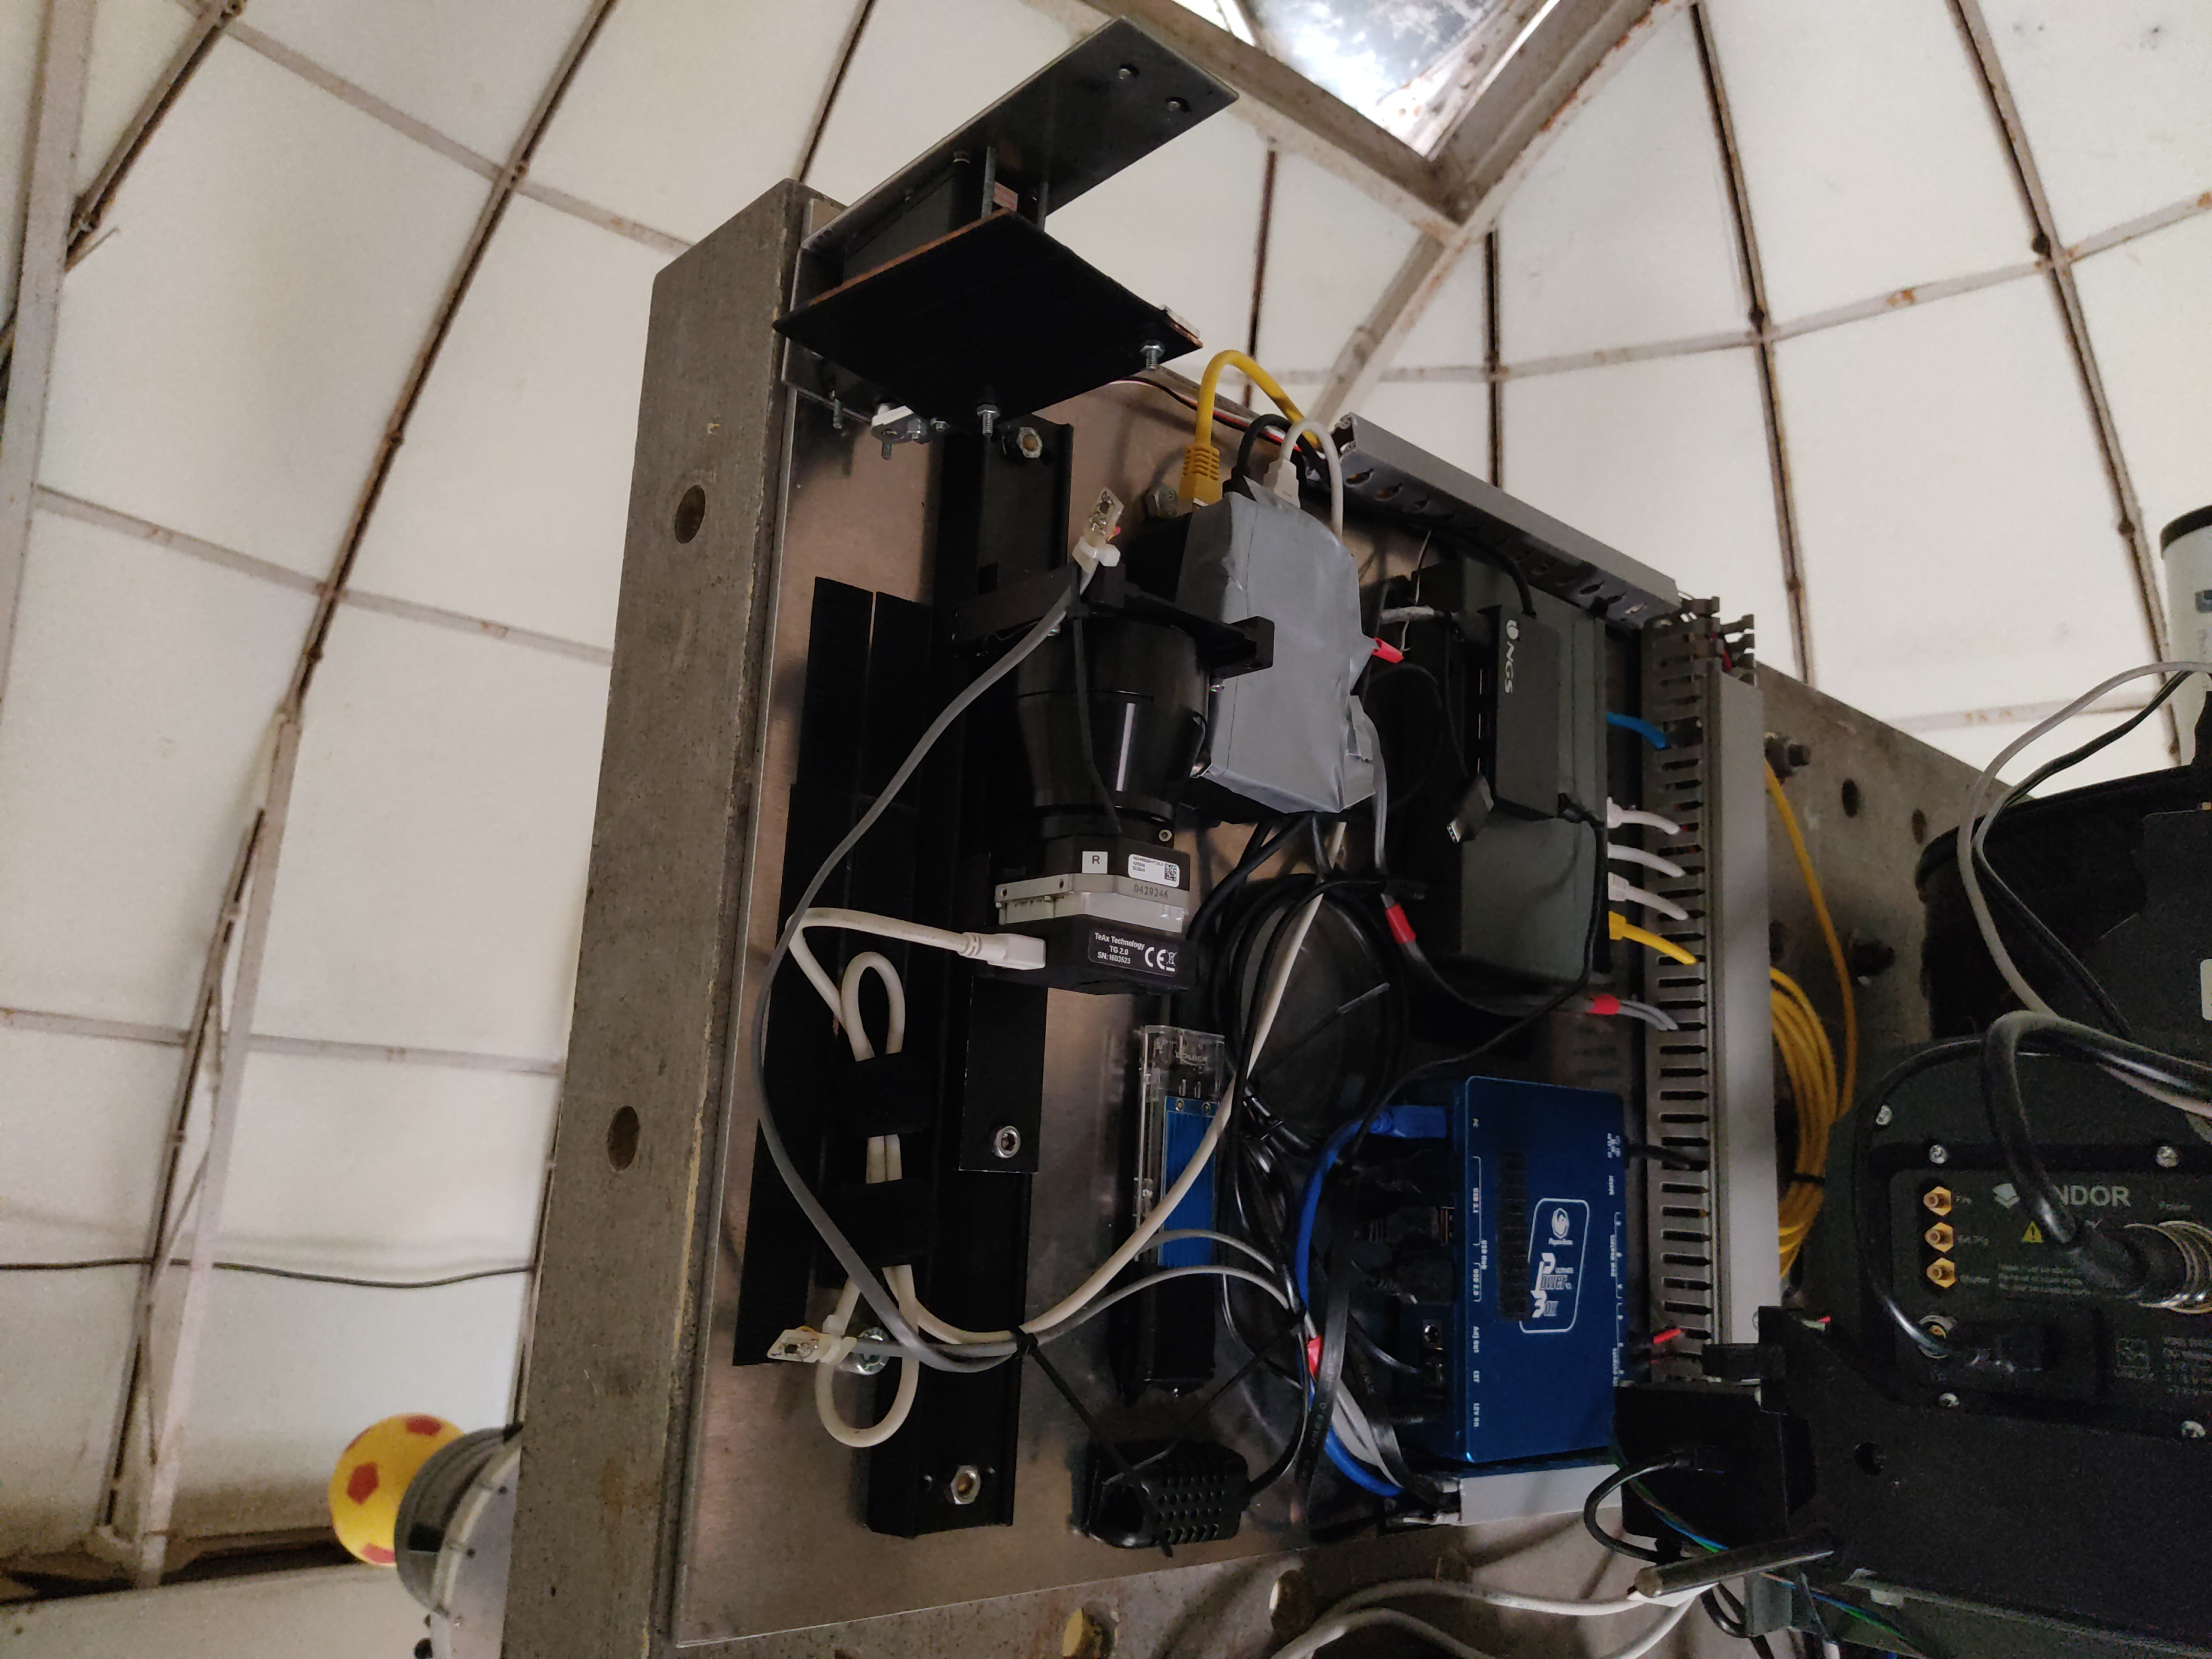
\includegraphics[width=\textwidth]{figures/infrared_instrument.pdf}
        %\caption{Subfigure 1}
        %\label{fig:subfig1}
    \end{subfigure}
    \hfill
    \begin{subfigure}[b]{\hsize}
        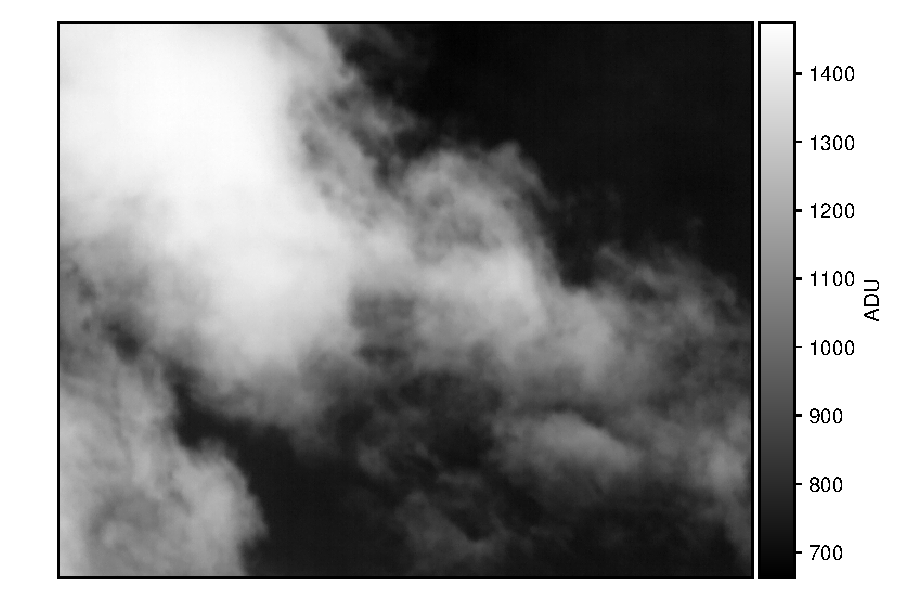
\includegraphics[width=\textwidth]{figures/sample_sky_image.pdf}
        %\caption{Subfigure 2}
        %\label{fig:subfig2}
    \end{subfigure}
    \caption{\textit{Top:} infrared instrument installed onto the equatorial table of the StarDICE experiment at Observatoire de Haute-Provence. \textit{Bottom:} sample of raw infrared thermal image.}
    \label{fig:infrared_system}
\end{figure}


%\subsection{Extraction of sky/cloud data from LWIR images}

%Infrared radiation has been recognized as holding significant promise in yielding valuable insights into cloud properties and atmospheric information. The 8–14 $\mu m$ spectral range - specifically the 10-12 $\mu m$ sometimes called the \textit{transparency window} - is characterized by minimal atmospheric emission and absorption. Radiative simulations of the atmosphere with \textsc{libRadTran} can provide a clearer depiction of the atmospheric window's attributes (e.g, sky downwelling radiance spectrum, transmittance, emittance). Figure \ref{} illustrates one typical simulation with different atmosphere reference models in the LWIR. Curves may be shifted up or down as a function of the zenith angle $\theta_{z}$, the total quantity of ozone $O_{3}$, the precipitable water vapor (PWV) or the vertical aerosol optical depth (VAOD). We can denote high atmospheric transmittance and low atmospheric emission, apart from a region around 9.6 $\mu m$ due to ozone (O3) absorption.

%Sky radiance emitted by the atmosphere is primarily controlled by water vapor content and clouds. During clear-sky/cloud-free conditions, the radiation received at the ground is both minimal and subject to fluctuations based on the quantity of water vapor present. Previous investigations have demonstrated a quadratic relationship between downwelling infrared radiation and the amount of precipitable water vapor (PWV). 

\subsection{Datasets and pre-processing}

Large number of images are required to properly train and test the classifier and segmentation algorithms. Our dataset consists of self-captured LWIR sky images. They consists of XXX sky images captured by the infrared thermal camera. Original-sized images (640 $\times$ 512) have been binned in 4$\times$4 format to be 160 $\times$ 128 resolution to accelerate computation and minimize memory usage.Cloudy sky images were collected over a period of 3 nights at Observatoire de Haute-Provence in January 2023 (43° 55' 51" N, 5° 42' 48" E). Cloud-free images were collected over a short period of time during the same month.

However, to compensate for the lack of cloud-free images and prevent any bias during training due to the data imbalance, we generate synthetic cloud-free images to form a composite cloud-free dataset containing as much images as the cloudy dataset. Synthetic images reproduce realistic observations by generating 2D horizontal gradient based images simulating increase in sky downwelling radiance as the camera FOV tilts towards high zenith angles (i.e, low elevation angles). Realistic sources of noises affecting uncooled infrared thermal cameras are introduced, including: read noise, fixed pattern noise, sky noise and narcissus effect. These are added so that the image spatial noise is equivalent to true cloud free images. Figure \ref{fig:synthetic_clear_sky_image} depicts one typical cloud-free image and a synthetic generated one with the spatial noise denoted for each of them. Note that the absolute ADU value has no impact as data is normalized prior to training.

\begin{figure}[t]
	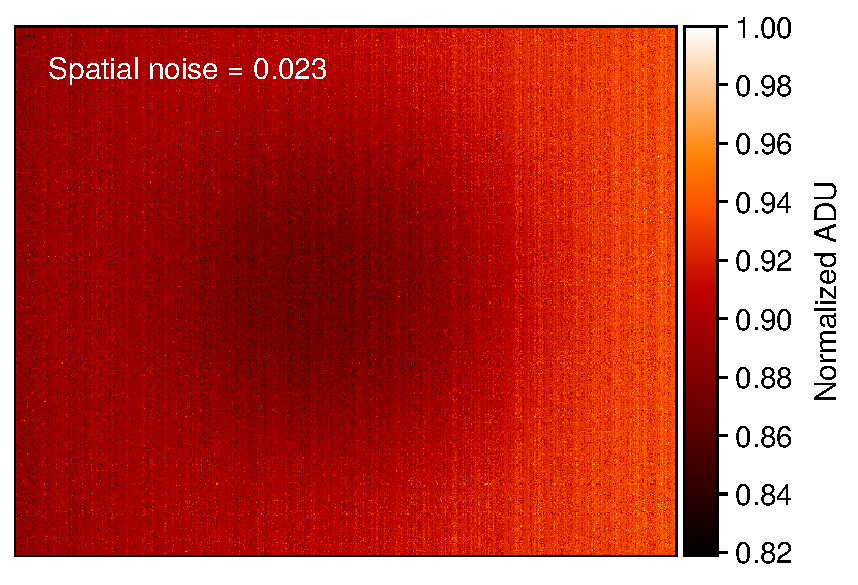
\includegraphics[width=\hsize]{figures/synthetic_clear_sky_image.pdf}
	\caption{Comparison between real observed clear sky image (top) and synthetically generated realisitic image (bottom). Spatial noise is marked on the top right corner of each image.}
    \label{fig:synthetic_clear_sky_image}
\end{figure}

All images and masks are visually inspected. Samples presenting artifacts such as tree branches from surroundings or building in the corner FOV are discarded. As the camera acquisition framerate enables to record up to 9 images per second, the pre-processing algorithm included constraints on consecutive image selection based on their timeseries. Selected frames are taken from at least 2 seconds between each other.

Ground-truth masks identifying cloud structure on cloud images were manually created through multiple steps of stretching procedures using \textsc{astropy} methods. They consist of boolean 2D array of the same image size, where \textit{True} identified pixels represent cloud pixels and \textit{False} identified pixels represent clear sky areas. This step could not be automated as cloud optical depths differ significantly. Indeed, the segmentation model aims at automating this tedious time consuming operation in real-time during observations. Figure \ref{fig:cloud_images_ground_truth} depicts two raw images with their associated manually generated ground-truth cloud masks for training purposes.

\begin{figure}[t]
	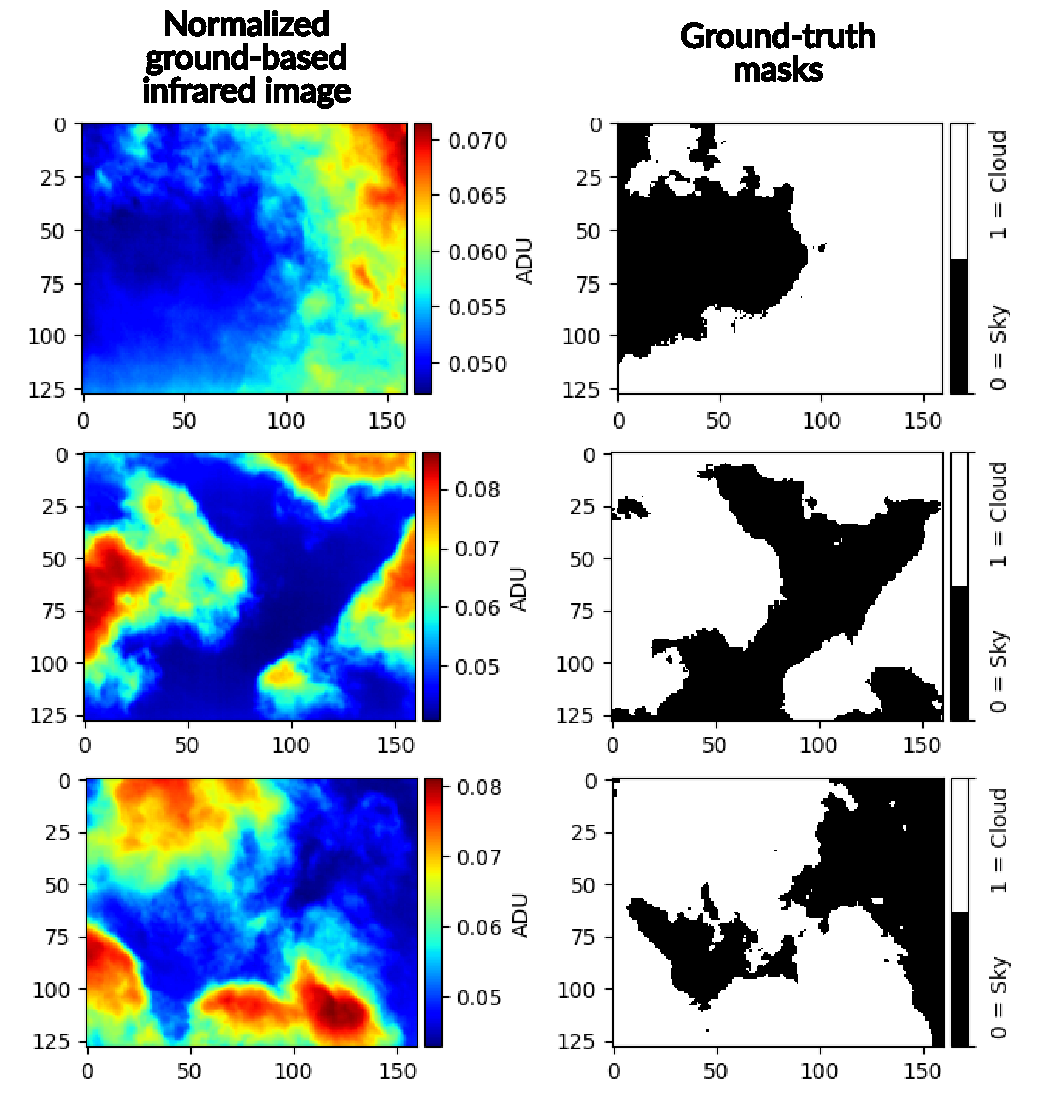
\includegraphics[width=\hsize]{figures/cloud_images_ground_truth.pdf}
	\caption{Representative infrared cloudy sky images and their corresponding manually created ground-truth masks. The masks are binary images, where zero represents clear sky and one represents cloud.}
    \label{fig:cloud_images_ground_truth}
\end{figure}

Furthermore, we performed multiple random augmentations (e.g, flip, shear, rotate, shift and zoom) on each original image to double the size of each dataset. All augmented images are produced through the random sequential applications of these five distinct operations to initial images.
These operations are executed with a random varying degree of intensity contained in specific ranges. Random rotations are applied within an amplitude ranging from -45 to +45 degrees. Shear is introduced with a random magnitude ranging from -0.2 to +0.2. Shifting operations are carried out with a maximum ratio of 10\% in both width and height directions to avoid generation of unrealistic symmetric structures. Zoom operation is applied within the range of 1 to 1.8. No other transformation such as histogram equalization or contrast enhancment is applied to prevent any bias or alteration in the segmentation performance. After the selection and augmentation procedures, we conducted a visual examination of all the created sky/cloud images to ensure that they appear realistic. Since all the parameters in the image augmentation process undergo controlled adjustments, our generated images closely mirror authentic sky/cloud scenes.

Datasets are for both models are splitted into training, testing and validation subsets with ratio of in the ratio of 70\%, 20\% and 10\% respectively.

\begin{table}[t]
\begin{center}
    \caption{Overview of the collected image datasets for classification and segmentation.}
    \begin{tabular}{c c c c} 
        \tophline
     Image type & \# training & \# validation & \# total \\ [1.0ex]
     \hline
     Clear & XXXX & XXXX & XXXX \\ [1.0ex]
     \hline
     Cloud & XXXX & XXXX & XXXX \\ [1.0ex]
     \hline
    \end{tabular}
    \belowtable{}
    \end{center}

\end{table}

\section{Image classification and cloud structure detection framework}

\subsection{Overall framework of IRIS-CloudDeep}

In this section, we outline the architectural designs of two distinct deep-learning models tailored for cloud-related tasks. On the one hand, we implement a classifier for cloud classification using Convolutional Neural Networks (CNN) \citep{lecun1995convolutional, Krizhevsky2012}, whose only goal is to discriminate between cloud-free and cloudy images. On the other hand, the segmentation for cloud structure detection is performed via the U-Net model \citep{UNET}. The output probability map can later be thresholded according to the user needs in order to produce the desired predicted binary segmentation map. Figure \ref{fig:architecture_schematic} illustrates the proposed deep-learning framework compared to conventional segmentation algorithms.

\begin{figure*}[t]
	\includegraphics[width=\hsize]{figures/architecture_schematic-crop.pdf}
	\caption{Schematic diagram of common-used deep-learning architectures (top) and this paper solution (bottom). The input image is a 160 × 128 radiometric grayscale image of the sky from the LWIR instrument. Classifier model output is a boolean.}
    \label{fig:architecture_schematic}
\end{figure*}


\subsection{Image classification}

For our image classification model, we employed a Convolutional Neural Network (CNN) architecture derived from the VGG-16 network \citep{simonyan2015deep}, which has proven to be highly effective in image recognition tasks \citep{ canziani2016analysis}. This modified network was designed with the primary objective of distinguishing between images that contain clouds and those that do not and is similar to SegCloud \citep{SegCloud}. Figure \ref{fig:schematics_classification_model} depicts the schematic of the architecture.

The VGG-16 architecture serves as the backbone of our model, providing a robust foundation for feature extraction. It consists of a series of convolutional layers, followed by rectified linear unit (ReLU) activation \citep{agarap2018deep} and max-pooling operations. This configuration facilitates the  extraction of hierarchical features that are pivotal for accurate classification. We retained the convolutional layers and their weight parameters from the original VGG-16 model to benefit from the network's ability to capture intricate visual patterns.

To adapt the network to our binary classification task, we made adjustments to the fully connected layers towards the end of the architecture. Specifically, we replaced the original fully connected layers with a custom set of fully connected layers. These modified layers were designed to map the learned features to the two classes of interest: images containing clouds and images without clouds. The final output layer consisted of two neurons, each representing one of the classes, and a softmax activation function was applied to obtain the class probabilities.

Furthermore, we incorporated dropout layers after the fully connected layers to mitigate overfitting and enhance the generalization capability of our model. This architectural modification helped us strike a balance between model complexity and performance, ensuring that the network could effectively differentiate between cloud and non-cloud images.

The model is trained on a comprehensive dataset encompassing both cloud and cloud-free infrared images, with corresponding ground truth labels.
 %The categorical cross-entropy loss function is employed for optimization, aiming to minimize the discrepancy between predicted and actual classifications.

\begin{figure*}[t]
	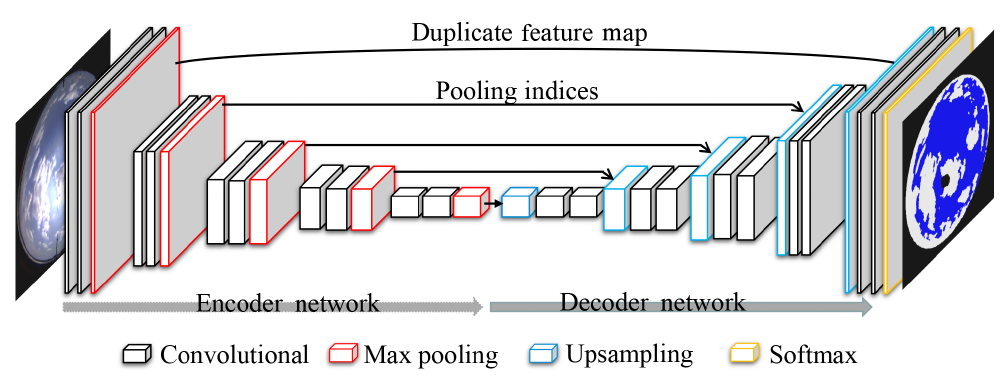
\includegraphics[width=\hsize]{figures/schematics_segmentation_model.png}
	\caption{
		Schematic diagram of the classifier model architecture. Boxes represent cross-sections of square feature maps.  The networks contain an encoder network, a corresponding decoder network, and a final Softmax classifier. Each map's dimensions are indicated on its lower left, and its number of channels are indicated above it. Half-grey boxes represent maps for which half of their channels are copied. The input image is a 160 × 128 radiometrically calibrated grayscale image of the sky from the LWIR instrument. Classifier model output is a boolean. Arrows represent operations, specified by the legend-notably, blue arrows represent convolutions, while gray ones represent copying (skip connections). Tensor dimensions at the output of each block are specified.}
        \label{fig:schematics_classification_model}
\end{figure*}

\subsubsection{Encoder block}

Our modified VGG-16-derived encoder comprises a stack of 10 convolutional layers and 5 max-pooling layers, each meticulously designed to facilitate feature extraction. Within each convolutional layer, a sequence of operations unfolds, encompassing convolution, batch normalization \citep{ioffe2015batch, bjorck2018understanding}, and rectified linear unit (ReLU) activation \citep{agarap2018deep}.

The initial step in this process is the convolution operation, where input feature maps are convolved with trainable filters featuring a 3$\times$3 window size and a stride of 1. Subsequently, batch normalization is employed to normalize the obtained feature maps. This normalization step is pivotal in accelerating the convergence of our model during training and counteracting issues related to the vanishing gradient problem.

Following batch normalization, ReLU activation is applied, introducing non-linearity into the network and expanding its capacity for feature representation. Notably, the early convolutional layers focus on capturing fine-grained visual details, such as shapes and edges, while the deeper convolutional layers leverage these foundational features to compute higher-level and more complex semantic characteristics, aligning with the principles elucidated by Liang et al. in 2017.

Additionally, our encoder network integrates 5 max-pooling layers, thoughtfully positioned after the convolutional layers. These layers play a pivotal role in enhancing the network's translation invariance, a critical characteristic for robust image classification. Each max-pooling layer performs subsampling on the input feature maps using a 2$\times$2 window size and a stride of 2, effectively reducing the size of output feature maps by half while capturing salient features. The incorporation of max-pooling layers further fortifies the network's ability to discern crucial information, ultimately contributing to the accuracy of our cloud image classification task.

\subsubsection{Decoder block}

The decoder network in our CNN classifier model, adapted from a modified VGG-16 architecture, plays a pivotal role in the restoration of high-level feature maps to the original image resolution, enabling precise cloud image classification.

Comprising 5 upsampling layers and 10 convolutional layers, the decoder network progressively increases the spatial resolution of feature maps while enhancing segmentation accuracy. Four of the upsampling layers utilize pooling indices from corresponding max-pooling layers in the encoder network, optimizing feature restoration with minimal computational overhead. However, this approach may slightly compromise cloud boundary details.

Recognizing the importance of preserving boundary information, the final upsampling layer employs a distinct strategy. It directly utilizes feature maps duplicated from the first max-pooling layers of the encoder network to improve cloud boundary recognition. This process involves bilinear interpolation, doubling the size of feature maps, and concatenating them with duplicated feature maps, ultimately achieving high-resolution cloud feature maps.

In summary, our decoder network systematically restores high-level cloud feature maps to the original image resolution through a series of upsampling layers. This process is vital for preserving details and enabling accurate cloud image classification within our modified VGG-16-based CNN classifier.

\subsubsection{Binary classifier}

The binary classifier is located after the decoder network to achieve final image classification. It is specifically designed for tasks where there are only two possible classes or categories, often labeled as "positive" and "negative" or "1" and "0.", in this case "cloud" or "clear". The classification process is realized through a sigmoid activation function. The output is a single-channel probability image, where each pixel's value is interpreted as the probability of it belonging to the cloud class. In practical terms, the pixel-wise predictions are obtained by applying a threshold to the probabilities. Pixels with probabilities exceeding a predefined threshold are classified as belonging to the cloud class, while those below the threshold are classified as non-cloud.


\subsection{Image segmentation}

For cloud structure identification, the U-Net architecture is adopted owing to its effifiency in semantic segmentation tasks. The U-Net model comprises an encoder and a decoder, facilitating the capturing of context-rich features and precise delineation of cloud structures. The encoder integrates convolutional and max-pooling layers to progressively downsample the input image, thereby capturing high-level features. These features are then decoded using up-convolutions and skip connections, enabling the reconstruction of the segmented cloud structures. Figure \ref{fig:schematics_segmentation_model} shows the architecture of the model and Figure \ref{fig:sample_segmentation} illustrates some examples of infrared cloud images and their corresponding ground-truth masks and predictions. 

\begin{figure*}[t]
    \centering
    
    \begin{subfigure}{\textwidth}
        \centering
        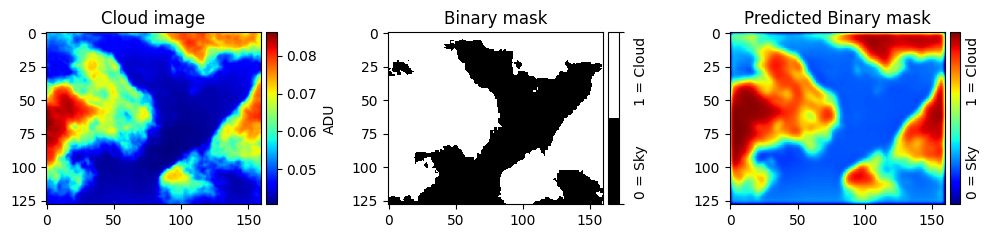
\includegraphics[width=1.0\linewidth]{figures/test_dl_15epochs.png}
        %\label{fig:sub1}
    \end{subfigure}
    
    \begin{subfigure}{\textwidth}
        \centering
        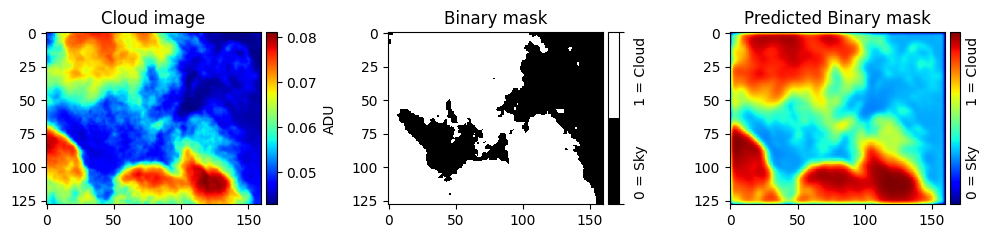
\includegraphics[width=1.0\linewidth]{figures/test_dl_15epochs2.png}
        %\label{fig:sub2}
    \end{subfigure}
    
    \begin{subfigure}{\textwidth}
        \centering
        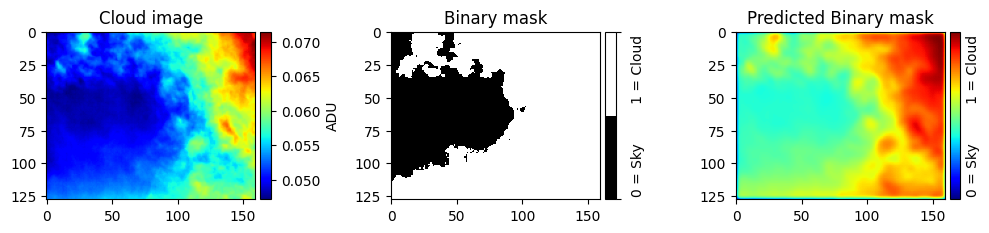
\includegraphics[width=1.0\linewidth]{figures/test_dl_15epochs3.png}
        %\label{fig:sub3}
    \end{subfigure}

    \caption{Sample of input images (left), associated ground-truth binary masks (center) and probabilistic map predictions (right) of IRIS-CloudDeep segmentation model.}
    \label{fig:sample_segmentation}
\end{figure*}

\begin{figure*}[t]
	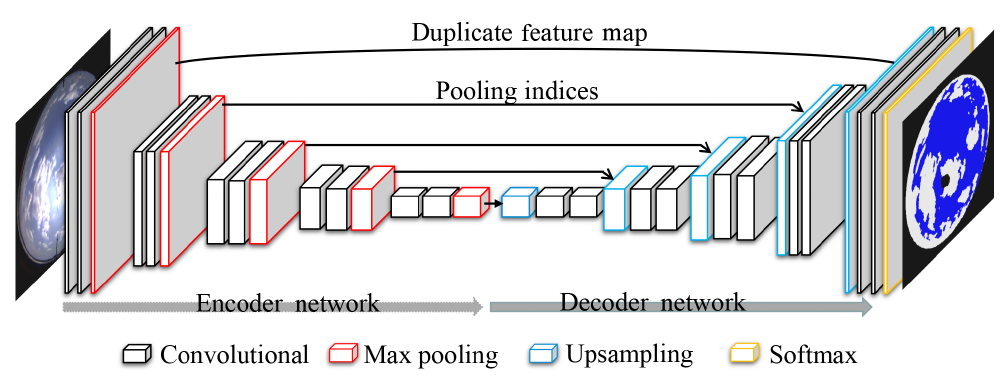
\includegraphics[width=\hsize]{figures/schematics_segmentation_model.png}
	\caption{
		Schematic diagram of U-Net based segmentation model architecture. Boxes represent cross-sections of square feature maps. The U-net model contains two parts: down-sampling (left half) and up-sampling (right half). After each convolutional layer, ReLU activation function (improves the computational speed of the training stage )and BN function were applied to effectively capture non-linearities in data and speedup the training
        Each map's dimensions are indicated on its lower left, and its number of channels are indicated above it. Half-grey boxes represent maps for which half of their channels are copied. The input image is a 160 × 128 radiometrically calibrated grayscale image of the sky from the LWIR instrument. The output image is a probabilistic mask prediction of pixels being cloudy or clear. Arrows represent operations, specified by the legend-notably, blue arrows represent convolutions, while gray ones represent copying (skip connections). Tensor dimensions at the output of each block are specified. Classifier model output is a boolean.}
    \label{fig:schematics_segmentation_model}
\end{figure*}

\subsubsection{Encoder block}

The encoder block of IRIS-CloudDeep segmentation model consists of four convolution layers and four max-pooling layers. We feed a normalized and binned 4x4 radiometrically calibrated image of a fixed input size (160 × 128 pixels) into the model.
The initial convolutional layer applies a set of learnable filters to the input image, extracting low-level features. Additional convolutional layers increase the complexity of learned features by applying convolutions to the feature map generated by the previous layer, creating a hierarchy of increasingly abstract features. After a set of convolutional layers, a max-pooling layer is applied to downsample the feature map. Max-pooling helps to reduce the spatial dimensions of the feature map while retaining the most salient information.

\subsubsection{Decoder block}

The decoder takes the high-level features generated by the encoder and aims to restore the spatial resolution of the original input image. In the U-Net architecture, the decoder is connected to the encoder via skip connections, enabling the network to combine local and contextual information. The decoder starts with an upsampling operation to increase the spatial dimensions of the feature map. A skip connection connects the upsampled feature map from the decoder with the corresponding feature map from the encoder. This enables the network to leverage both local and global context information. Following the concatenation, a series of convolutional layers are applied. These layers refine the combined feature map, gradually transitioning from abstract features to more detailed information. The final convolutional layer produces the segmentation mask of the U-Net model.

\subsubsection{Model output}

The output the classifier is a boolean representing whether the image contains cloud or not. On the contrary, the image segmentation model output is a probability mask that assigns a probability value to individual pixels, indicating their potential belonging in the cloud category.
 %Subsequently, a straightforward thresholding technique is applied to transform the probability mask into a binary map. The threshold for labeling is obtained from the Receiver Operating Curve (ROC) analysis specific to our experimental conditions.

\subsection{Training procedure and implementation details}

%\subsubsection{Loss function}
The CNN classifier is trained on the dataset containing both cloudy and synthetic clear sky images. The U-Net model is trained on cloudy images only which is the labeled dataset containing infrared images with pixel-wise cloud structure annotations (ground-truth masks). The loss function employed for training is the binary cross-entropy, which quantifies the difference between predicted probabilities and actual binary class labels for each instance in the dataset. Mathematically, given an instance's true binary label $y$ (0 or 1) and the predicted probability $p$ of it belonging to class 1, the binary cross-entropy loss $\mathcal{L}$ is calculated as:
\begin{equation}
	\mathcal{L} = -\frac{1}{N}\sum_i y_i\cdot\log\left(f_w(x_i)\right) + (1-y_i)\cdot\log\left(1-f_w(x_i)\right)
\end{equation}
where $\mathcal{L}$ is the binary cross-entropy loss. $N$ is the total number of instances in the dataset, $i$ index represents an individual instance, $y_{i}$ is the $i$-th true binary label (0 or 1) and $f_w(x_i)$ is the predicted probability that belongs to class 1, based on the model with parameters $w$. The goal of training is to minimize this loss function by adjusting the model parameters weights $w$ to better align the predicted probabilities $f_w(x_i)$ with the true labels $y_{i}$.

Both architectures are implemented in \textsc{Python} with the \textsc{keras}\footnote{\url{https://keras.io}} \citep{Keras} subpackage of \textsc{TensorFlow}\footnote{\url{https://www.tensorflow.org}} framework \citep{TensorFlow}. IRIS-CloudDeep is trained on the GPU cluster infrastructure of the MESO@LR\footnote{\url{https://meso-lr.umontpellier.fr/}} high-performance computing center. Images are normalized and binned into a fixed 160 $\times$ 128 resolution format to speed up computations and to capture the global trend. Models are trained over 500 and 1000 epochs respectively using the ADAM optimizer \citep{ADAM}. We set the batch size to 16 images with a dynamic learning rate initial value of $\lambda$ = 0.001 that decreases through the training epochs following the relation : $\lambda(\text{epoch}) = 0.001 \cdot 0.5^{\left\lfloor \frac{\text{epoch}}{10} \right\rfloor}
$. We also set an earlystopping watchdogs that interrupts the training if the loss value doesn't decrease below a certain threshold after 15 epochs.  Hyperparameters are fine tuned with the \textsc{optuna}\footnote{\url{https://optuna.org/}} hyperparameter optimization framework \citep{Optuna} using the sampling strategy algorithm.

\section{Experiments}

\subsection{Performance metrics}

In order to evaluate the performance of the proposed models, we adopt six metrics: precision (P), accuracy (A), recall (R), F1-score (F1), intersection over union (IoU) and error rate (ER) between the ground-truths and the predictions. For the segmentation model, accuracy and interesection over union are averaged over the pixels to get the mean pixel accuracy (mA) and the mean intersection over union (mIoU). All of these parameters are defined in the following equations,
\begin{equation}
    P = \frac{TP}{TP + FP}
\end{equation}
\begin{equation}
    A = \frac{TP + TN}{TP + TN + FP + FN}
\end{equation}
\begin{equation}
    R = \frac{TP}{TP + FN}
\end{equation}
\begin{equation}
    F1 = \frac{2 \cdot P \cdot R}{P + R}
\end{equation}
\begin{equation}
    IoU = \frac{TP}{TP + FP + FN}
\end{equation}
\begin{equation}
    ER = \frac{FP + FN}{TP + TN + FP + FN}
\end{equation}
with True Positives (TP) the number of correctly classified positive instances; False Positives (FP) the number of negative instances that were incorrectly classified as positive; False Negatives (FN) the number of positive instances that were incorrectly classified as negative; True Negatives (TN) the number of correctly classified negative instances.

\subsection{Framework effectiveness}

\textcolor{red}{The trend of binary cross-entropy loss for training and testing sets are shown in Fig. 2. We observe that the loss saturates after
a few thousand iterations, and the model exhibits comparable
loss performance for both training and testing sets. We choose
the CloudSegNet model with the lowest validation loss for our
subsequent experiments.As discussed above, the output of CloudSegNet is a prob-ability mask, wherein each pixel indicates the degree of belongingness to the cloud category. Since the ground-truth maps are binary in nature, it is necessary to convert the probabilistic output into binary maps as well. We employ a Receiver Operating Curve (ROC) technique to understand the impact of the threshold on the performance. We vary the threshold from 0 to 1 in steps of 0.01, and record the False Positive Rate (FPR) and True Positive Rate (TPR) of cloud detection. Figure 3 shows the resulting ROC curve. The area under the ROC curve (AUC) is 0.97, indicating the competitive performance of CloudSegNet. The ROC curve provides an opportunity to choose a threshold, based on the trade-off between FPR and TPR. In our experiments, we choose the threshold of 0.5 to convert the probabilistic map into a binary sky/cloud image, which is very close to equal true and false positive rates. Of course, this threshold can be further adjusted by the user, based on the specific requirements for TPR and/or FPR. Figure 4 shows some sample outputs of our proposed approach. Visual inspection of additional images from our SWINySeg dataset confirms that CloudSegNet can successfully identify cloud pixels from nychthemeron images.}

\begin{figure}[t]
	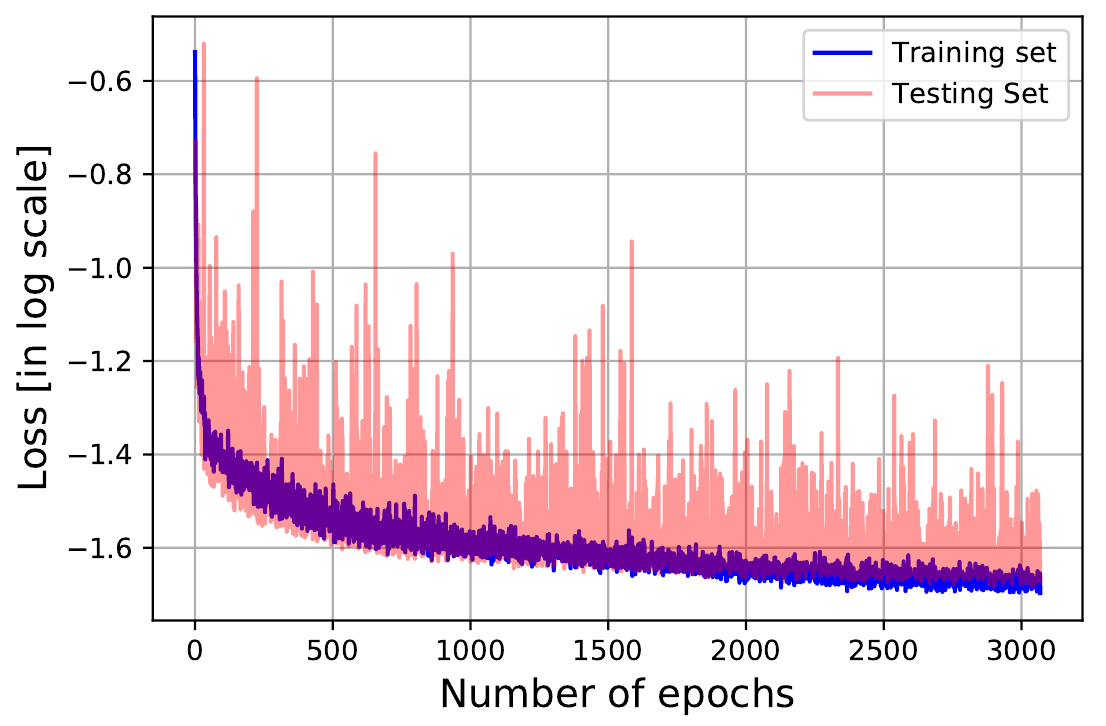
\includegraphics[width=\hsize]{figures/loss_trend.png}
	\caption{Training and testing losses of IRIS-CloudDeep models over
    epochs. The dashed curve is for training whereas the continuous curve is for testing. Blue and red curves denote the classifier and segmentation models respectively.}
    \label{fig:loss_trend}
\end{figure}

\textcolor{red}{Table 1 reports that SegCloud achieves a high average ac-
curacy of 96.24\%, which further objectively proves its effec-
tiveness. Moreover, SegCloud performs well on whole-sky
images with different cloud cover conditions and achieves
96.98\% accuracy on clear-sky images, 95.2\% accuracy on
partial-cloud images, and 99.44\% near-perfect accuracy on overcast-sky images. These experimental results show that
the SegCloud is effective and accurate for cloud segmenta-
tion and can provide a reference for future cloud segmenta-
tion research.}

\begin{table*}[t]
\begin{center}
    \caption{Evaluation metrics for comparison of segmentation models performances on the self-capture testing set. Best values are denoted in bold font. (P = precision, mPA = mean pixel accuracy, R = recall, F1 = F1-score, mIoU= mean intersection over union, ER = error-rate)}
    \begin{tabular}{c c c c c c c} 
    \tophline \hline
     Model & P [\%] & mPA [\%] & R & F1 [\%] & mIoU [\%] & ER [\%] \\ [1.0ex]
     \hline
     SegNet & XXXX & XXXX & XXXX & XXXX & XXXX & XXXX \\ [1.0ex]
     CloudDeepLabV3+ & XXXX & XXXX & XXXX & XXXX & XXXX & XXXX \\ [1.0ex]
     CloudSegNet & XXXX & XXXX & XXXX & XXXX & XXXX & XXXX \\ [1.0ex]
     CloudUNet & XXXX & XXXX & XXXX & XXXX & XXXX & XXXX \\ [1.0ex]
     CloudUNetv2 & XXXX & XXXX & XXXX & XXXX & XXXX & XXXX \\ [1.0ex]
     PSPNet & XXXX & XXXX & XXXX & XXXX & XXXX & XXXX \\ [1.0ex]
     DeepCloud & XXXX & XXXX & XXXX & XXXX & XXXX & XXXX \\ [1.0ex]
     TransCloudSeg & XXXX & XXXX & XXXX & XXXX & XXXX & XXXX \\ [1.0ex]
     \textbf{IRIS-CloudDeep} & XXXX & XXXX & XXXX & XXXX & XXXX & XXXX \\
     \hline
    \end{tabular}
    \belowtable{}
    \end{center}
\end{table*}

\subsubsection{Classifier}

\subsubsection{Segmentation}

\subsection{Comparison of segmentation model performance with other methods}

\begin{figure}[t]
	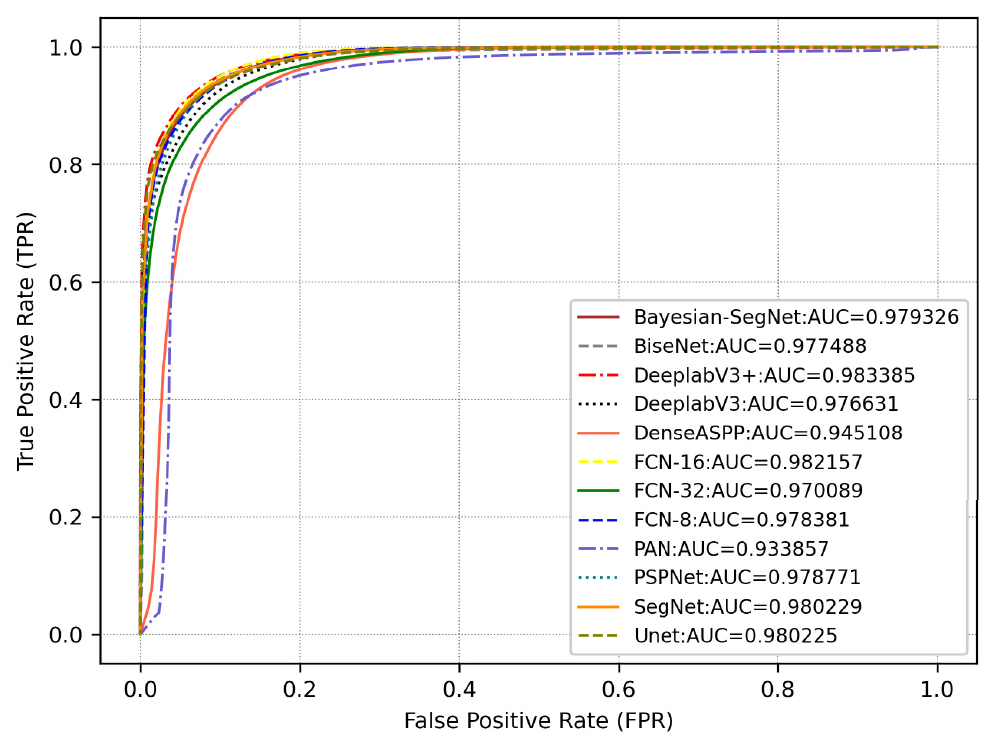
\includegraphics[width=\hsize]{figures/roc_curve.png}
	\caption{ROC curve comparison of different segmentation models. The AUC value represents the area under the curve.}
    \label{fig:roc_curve}
\end{figure}

\textbf{Insist on the non-feasibility to compare to traditional methods properly as they rely on color information from red and blue channels.}

\textcolor{red}{To accurately measure the segmentation performance of the CloudDeepLabV3+ on the ground-based cloud image, this study is compared with other models (CloudSegNet, U-Net (Ronneberger, Fischer, and Brox 2015), PSPNet (Zhao et al. 2017), SegCloud, CloudU-Net, CloudU-Netv2 and DeepLabV3+) on the SWINySEG dataset, as shown in Table 6.
The indicators of CloudSegNet are the worst, with Accuracy, mPA, F1-Score, and mIoU failing to reach 90\%, and Error Rate exceeding 10\%. U-Net, PSPNet, SegCloud, and DeepLabV3+ have similar segmentation data, and mIoU is 90\%, approximately. The segmentation data indicators of CloudU-Net and CloudU-Netv2 are better. Accuracy, mPA, and F1-Score all exceed 96\%, and mIoU reaches 92.90\% and 93.42\%, respectively. The CloudDeepLabV3+ proposed in this study has the best effect, and the five evaluation metrics are superior to other models. The key mIoU is 0.88\% higher than the state-of-the-art cloud segmentation method CloudU-Netv2. In addition, other indicators are about 0.42\% higher than CloudU-Netv2, and the error rate is reduced by 0.49\%. Figure 10 shows the segmentation results of different models in the form of histograms. We choose the parameters such as floating point operations (FLOPs), training time, and testing time to evaluate the computational complexity of different models. As shown in Table 7, the state-of-the-art cloud segmentation CloudU-Netv2 spends more time than CloudDeepLabV3+, and the parameters and FLOPs are much more. Compared with other models, our model has a lower computational complexity and has more advantages. Therefore, CloudDeepLabV3+ is the optimal choice for cloud image segmentation. It provides a substantial performance improvement and achieves excellent and more competitive cloud image segmentation results with less model complexity.}

We use this augmented composite datasets of 10,000 images respectively to train the classifier and identifer. Random sampling is applied on each composite dataset, and standard train-test-validation split is perormed . Figure \ref{} depicts trends for the binary cross-entropy losses for training and testing subsets with various hyperparameters. \textsc{Optuna} framework allows ease of hyperparameters optimization. We observe that the loss saturates after a few hundred iterations for all attempts, and the model exhibits comparable loss performance for both training and testing sets. We select the model and layer parameters with the lowest validation loss for our subsequent experiments.

\subsection{Performance}



Results are summarized in Table \ref{}. The purity is also
very high, with a value of 98.5. For classificatoin, the model reaches high performance of XXX accuracy and XXX YYY. We measure a completeness of 87 and a purity of 93.6. Our cloud structure identification model reaches an IoU above 0.8 at any magnitude, and up to 0.9 for bright objects (small magnitude).

\section{Discussion}

\subsection{Evaluating segmentation model onto other datasets}

\textcolor{red}{Strong generalization ability and robustness are also quite
indispensable attributes of a state-of-the-art model. Therefore,
The Cirrus Cumulus Stratus Nimbus (CCSN) data set and the
UTILITY data set were put into the TL-DeepLabV3+. A few
samples of segmentation results were visualized in Fig. 4. The
results show that most of the clouds in the images can be
accurately recognized by the model, such as the first column
and second column in Fig. 4(a) and (b). Especially the picture
in the fourth column of Fig. 4 obtains nearly perfect perfor-
mance. The high-accuracy prediction results can be processed
to the cloud masks of these nonannotated data sets, increasing
the amount of labeled cloud segmentation data sets. For those
images that contain elements other than clouds or sky [left
three columns in Fig. 4(a)], the model keeps a relatively
accurate recognition rate for the parts of cloud and sky.
However, the other elements such as mountains and vegetation
are obviously misjudged by the model because the GBCS data
set only includes sky and clouds, and the model does not learn
the features of other elements. The image in the third column
of Fig. 4(c) has the worst performance in these samples. It may
be because this image is a nighttime cloud image with bad
illumination, which is not contained in the GBCS data set.
Thus, it is indispensable to add cloud images under diverse
light conditions in future data sets. Overall, the performance
on other data sets proves the excellent generalization ability
and robustness of TL-DeepLabV3+.}

\begin{table*}[t]
    \begin{center}
        \caption{Evaluation metrics for the proposed segmentation model on publicly available state-of-the-art datasets. Note that RGB color images are transformed into gray-scale images as IRIS-CloudDeep segmentation model is optimized for this type of data. Best values are denoted in bold font. (P = precision, mPA = mean pixel accuracy, R = recall, F1 = F1-score, mIoU= mean intersection over union, ER = error-rate)}
        \begin{tabular}{c c c c c c c} 
        \tophline \hline
         Dataset & P [\%] & mPA [\%] & R & F1 [\%] & mIoU [\%] & ER [\%] \\ [1.0ex]
         \hline
         SWIMSEG & XXXX & XXXX & XXXX & XXXX & XXXX & XXXX \\ [1.0ex]
         SWINSEG & XXXX & XXXX & XXXX & XXXX & XXXX & XXXX \\ [1.0ex]
         SWINySEG & XXXX & XXXX & XXXX & XXXX & XXXX & XXXX \\ [1.0ex]
         WSISEG & XXXX & XXXX & XXXX & XXXX & XXXX & XXXX \\ [1.0ex]
         HYTA & XXXX & XXXX & XXXX & XXXX & XXXX & XXXX \\ [1.0ex]
         TLCDD & XXXX & XXXX & XXXX & XXXX & XXXX & XXXX \\ [1.0ex]
         \textbf{Paper dataset} & XXXX & XXXX & XXXX & XXXX & XXXX & XXXX \\
         \hline
        \end{tabular}
        \belowtable{}
        \end{center}
    \end{table*}

\subsection{Comparison to Otsu method}

\textcolor{red}{The Otsu algorithm has poor
performance in segmenting whole-sky images because it re-
quires pixels of the same class to have a similar gray value,
but clouds exhibit the opposite behavior. The R/B threshold
method has more accurate segmenting results compared with
the Otsu algorithm. However, segmenting accuracy is poor
especially for circumsolar areas (Fig. 4a, b and c) because
circumsolar areas often have texture and intensity similar to
the clouds due to the forward scattering of visible light by
aerosols/haze and dynamic range limitation of the detectors
of the sky imager (Long and Charles, 2010). Thus, traditional
methods merely utilize low-level vision cues to segment im-
ages and tend to result in misclassification once the boundary
between clouds and sky is unclear. However, SegCloud per-
forms excellent segmentation compared with the two other
conventional methods and exhibits segmentation advantages
in the area near the sun. SegCloud learns from the given cal-
ibration database and constantly mines deep cloud features.
Thus, it has improved capability to identify circumsolar ar-
eas, although these pixels have textures and intensities that
are similar to those of clouds.
The average segmentation accuracy of the three algorithms
is also calculated on the test dataset to verify the performance
of the SegCloud objectively. Table 1 shows that SegCloud
obtains higher average accuracy than the two other methods
do and achieves better segmentation performance for clear-
sky, partial-cloud, or overcast-sky images. Although Seg-
Cloud shows advantages in whole-sky image segmentation,
some misidentification remains due to decreased recognition
for extremely thin clouds, which should be investigated in
the future.}

\subsection{Future perspectives}

\conclusions  %% \conclusions[modified heading if necessary]

In this paper, we proposed IRIS-CloudDeep, a deep-learning framework for classification and segmentation of LWIR
ground-based thermal images. As far as we know, it is the framework that attempts to apply two sequential models for complementary tasks on single-channel gray-scaled infrared images. Specifically, we presented the CNN-based classifier and the U-Net based segmentation model tailored to extract cloud structures on pre-identified cloud images. Extensive experimental results on a combination of self-acquired data and transformed publicly available datasets have demonstrated
the effectiveness and performances of the proposed framework. We successfully increased the size of training, testing and validation subsets with random application of augmentation methods. We developed an accurate simulation tool to produce realistic clear sky images. In the future, additional data will be collected by the infrared instrument, capturing various weather conditions. The framework may be re-trained on heavier datasets that will probably increase its accuracy.  Furthermore, if enough data is collected with many different cloud categories, we will be able to modify the segmentation model to perform cloud typology. Finally, the current trained model is expected to process data in real-time for the StarDICE experiment in order to: (i) give live alerts to remote observers in the case of cloud detection; (ii) set a flag in CCD images for quality sorting in post-processing.


%% The following commands are for the statements about the availability of data sets and/or software code corresponding to the manuscript.
%% It is strongly recommended to make use of these sections in case data sets and/or software code have been part of your research the article is based on.





%\codeavailability{TEXT} %% use this section when having only software code available

%\dataavailability{} %% use this section when having only data sets available

\codedataavailability{The code is freely available online at \url{https://github.com/kelian98/IRIS-CloudDeep}. The datasets will be made available from authors Kélian Sommer (kelian.sommer@umontpellier.fr) and corresponding author Wassim Kabalan (wassim.kabalan@apc.in2p3.fr) upon request.} %% use this section when having data sets and software code available

\authorcontribution{KS conceived the instrument, collected data and pre-process the dataset by creating ground truths masks for segmentation and producing realistic synthetic data for classification. WK, RB and KS designed the framework. WK and RB performed the experiments. KS wrote the paper and collected relevant literature. WK and RB revised the manuscript; AB, JCT and BP proposed constructive suggestions on the revision of the article.} %% this section is mandatory

\competinginterests{The authors declare that they have no conflict of interest.} %% this section is mandatory even if you declare that no competing interests are present

%\disclaimer{TEXT} %% optional section

\begin{acknowledgements}
This work has been realized with the support of MESO@LR-Platform at the University of Montpellier.
\end{acknowledgements}


%sampleavailability{TEXT} %% use this section when having geoscientific samples available

%\videosupplement{TEXT} %% use this section when having video supplements available


%\appendix
%\section{}    %% Appendix A

%\subsection{}     %% Appendix A1, A2, etc.


%\noappendix       %% use this to mark the end of the appendix section. Otherwise the figures might be numbered incorrectly (e.g. 10 instead of 1).

%% Regarding figures and tables in appendices, the following two options are possible depending on your general handling of figures and tables in the manuscript environment:

%% Option 1: If you sorted all figures and tables into the sections of the text, please also sort the appendix figures and appendix tables into the respective appendix sections.
%% They will be correctly named automatically.

%% Option 2: If you put all figures after the reference list, please insert appendix tables and figures after the normal tables and figures.
%% To rename them correctly to A1, A2, etc., please add the following commands in front of them:

\appendixfigures  %% needs to be added in front of appendix figures

\appendixtables   %% needs to be added in front of appendix tables

%% Please add \clearpage between each table and/or figure. Further guidelines on figures and tables can be found below.








%% REFERENCES

%% The reference list is compiled as follows:

%\begin{thebibliography}{}

%\bibitem[AUTHOR(YEAR)]{LABEL1}
%REFERENCE 1

%\bibitem[AUTHOR(YEAR)]{LABEL2}
%REFERENCE 2

%\end{thebibliography}

%% Since the Copernicus LaTeX package includes the BibTeX style file copernicus.bst,
%% authors experienced with BibTeX only have to include the following two lines:
%%

%\bibliographystyle{abbrv}
\bibliography{biblio.bib}
%%
%% URLs and DOIs can be entered in your BibTeX file as:
%%
%% URL = {http://www.xyz.org/~jones/idx_g.htm}
%% DOI = {10.5194/xyz}


%% LITERATURE CITATIONS
%%
%% command                        & example result
%% \citet{jones90}|               & Jones et al. (1990)
%% \citep{jones90}|               & (Jones et al., 1990)
%% \citep{jones90,jones93}|       & (Jones et al., 1990, 1993)
%% \citep[p.~32]{jones90}|        & (Jones et al., 1990, p.~32)
%% \citep[e.g.,][]{jones90}|      & (e.g., Jones et al., 1990)
%% \citep[e.g.,][p.~32]{jones90}| & (e.g., Jones et al., 1990, p.~32)
%% \citeauthor{jones90}|          & Jones et al.
%% \citeyear{jones90}|            & 1990



%% FIGURES

%% When figures and tables are placed at the end of the MS (article in one-column style), please add \clearpage
%% between bibliography and first table and/or figure as well as between each table and/or figure.

% The figure files should be labelled correctly with Arabic numerals (e.g. fig01.jpg, fig02.png).


%% ONE-COLUMN FIGURES

%%f
%\begin{figure}[t]
%\includegraphics[width=8.3cm]{FILE NAME}
%\caption{TEXT}
%\end{figure}
%
%%% TWO-COLUMN FIGURES
%
%%f
%\begin{figure*}[t]
%\includegraphics[width=12cm]{FILE NAME}
%\caption{TEXT}
%\end{figure*}
%
%
%%% TABLES
%%%
%%% The different columns must be seperated with a & command and should
%%% end with \\ to identify the column brake.
%
%%% ONE-COLUMN TABLE
%
%%t
%\begin{table}[t]
%\caption{TEXT}
%\begin{tabular}{column = lcr}
%\tophline
%
%\middlehline
%
%\bottomhline
%\end{tabular}
%\belowtable{} % Table Footnotes
%\end{table}
%
%%% TWO-COLUMN TABLE
%
%%t
%\begin{table*}[t]
%\caption{TEXT}
%\begin{tabular}{column = lcr}
%\tophline
%
%\middlehline
%
%\bottomhline
%\end{tabular}
%\belowtable{} % Table Footnotes
%\end{table*}
%
%%% LANDSCAPE TABLE
%
%%t
%\begin{sidewaystable*}[t]
%\caption{TEXT}
%\begin{tabular}{column = lcr}
%\tophline
%
%\middlehline
%
%\bottomhline
%\end{tabular}
%\belowtable{} % Table Footnotes
%\end{sidewaystable*}
%
%
%%% MATHEMATICAL EXPRESSIONS
%
%%% All papers typeset by Copernicus Publications follow the math typesetting regulations
%%% given by the IUPAC Green Book (IUPAC: Quantities, Units and Symbols in Physical Chemistry,
%%% 2nd Edn., Blackwell Science, available at: http://old.iupac.org/publications/books/gbook/green_book_2ed.pdf, 1993).
%%%
%%% Physical quantities/variables are typeset in italic font (t for time, T for Temperature)
%%% Indices which are not defined are typeset in italic font (x, y, z, a, b, c)
%%% Items/objects which are defined are typeset in roman font (Car A, Car B)
%%% Descriptions/specifications which are defined by itself are typeset in roman font (abs, rel, ref, tot, net, ice)
%%% Abbreviations from 2 letters are typeset in roman font (RH, LAI)
%%% Vectors are identified in bold italic font using \vec{x}
%%% Matrices are identified in bold roman font
%%% Multiplication signs are typeset using the LaTeX commands \times (for vector products, grids, and exponential notations) or \cdot
%%% The character * should not be applied as mutliplication sign
%
%
%%% EQUATIONS
%
%%% Single-row equation
%
%\begin{equation}
%
%\end{equation}
%
%%% Multiline equation
%
%\begin{align}
%& 3 + 5 = 8\\
%& 3 + 5 = 8\\
%& 3 + 5 = 8
%\end{align}
%
%
%%% MATRICES
%
%\begin{matrix}
%x & y & z\\
%x & y & z\\
%x & y & z\\
%\end{matrix}
%
%
%%% ALGORITHM
%
%\begin{algorithm}
%\caption{...}
%\label{a1}
%\begin{algorithmic}
%...
%\end{algorithmic}
%\end{algorithm}
%
%
%%% CHEMICAL FORMULAS AND REACTIONS
%
%%% For formulas embedded in the text, please use \chem{}
%
%%% The reaction environment creates labels including the letter R, i.e. (R1), (R2), etc.
%
%\begin{reaction}
%%% \rightarrow should be used for normal (one-way) chemical reactions
%%% \rightleftharpoons should be used for equilibria
%%% \leftrightarrow should be used for resonance structures
%\end{reaction}
%
%
%%% PHYSICAL UNITS
%%%
%%% Please use \unit{} and apply the exponential notation


\end{document}
